%Power subsystem\documentclass[class=report,11pt,crop=false]{standalone}
% ----------------------------------------------------
% ----------------------------------------------------
\documentclass[class=report,11pt,crop=false]{standalone}
% Page geometry
\usepackage[a4paper,margin=20mm,top=25mm,bottom=25mm]{geometry}

% Font choice
\usepackage{lmodern}

\usepackage{lipsum}

% Use IEEE bibliography style
\bibliographystyle{IEEEtran}

% Line spacing
\usepackage{setspace}
\setstretch{1.20}

% Ensure UTF8 encoding
\usepackage[utf8]{inputenc}

% Language standard (not too important)
\usepackage[english]{babel}

% Skip a line in between paragraphs
\usepackage{parskip}

% For the creation of dummy text
\usepackage{blindtext}

% Math
\usepackage{amsmath}

% Header & Footer stuff
\usepackage{fancyhdr}
\pagestyle{fancy}
\fancyhead{}
\fancyhead[R]{\nouppercase{\rightmark}}
\fancyfoot{}
\fancyfoot[C]{\thepage}
\renewcommand{\headrulewidth}{0.0pt}
\renewcommand{\footrulewidth}{0.0pt}
\setlength{\headheight}{13.6pt}

% Epigraphs
\usepackage{epigraph}
\setlength\epigraphrule{0pt}
\setlength{\epigraphwidth}{0.65\textwidth}

% Colour
\usepackage{color}
\usepackage[usenames,dvipsnames]{xcolor}

% Hyperlinks & References
\usepackage{hyperref}
\definecolor{linkColour}{RGB}{77,71,179}
\hypersetup{
    colorlinks=true,
    linkcolor=linkColour,
    filecolor=linkColour,
    urlcolor=linkColour,
    citecolor=linkColour,
}
\urlstyle{same}

% Automatically correct front-side quotes
\usepackage[autostyle=false, style=ukenglish]{csquotes}
\MakeOuterQuote{"}

% Graphics
\usepackage{graphicx}
\graphicspath{{Images/}{../Images/}}
\usepackage{makecell}
\usepackage{transparent}

% SI units
\usepackage{siunitx}

% Microtype goodness
\usepackage{microtype}

% Listings
\usepackage[T1]{fontenc}
\usepackage{listings}
\usepackage[scaled=0.8]{DejaVuSansMono}

% Custom colours for listings
\definecolor{backgroundColour}{RGB}{250,250,250}
\definecolor{commentColour}{RGB}{73, 175, 102}
\definecolor{identifierColour}{RGB}{196, 19, 66}
\definecolor{stringColour}{RGB}{252, 156, 30}
\definecolor{keywordColour}{RGB}{50, 38, 224}
\definecolor{lineNumbersColour}{RGB}{127,127,127}
\lstset{
  language=Matlab,
  captionpos=b,
  aboveskip=15pt,belowskip=10pt,
  backgroundcolor=\color{backgroundColour},
  basicstyle=\ttfamily,%\footnotesize,        % the size of the fonts that are used for the code
  breakatwhitespace=false,         % sets if automatic breaks should only happen at whitespace
  breaklines=true,                 % sets automatic line breaking
  postbreak=\mbox{\textcolor{red}{$\hookrightarrow$}\space},
  commentstyle=\color{commentColour},    % comment style
  identifierstyle=\color{identifierColour},
  stringstyle=\color{stringColour},
   keywordstyle=\color{keywordColour},       % keyword style
  %escapeinside={\%*}{*)},          % if you want to add LaTeX within your code
  extendedchars=true,              % lets you use non-ASCII characters; for 8-bits encodings only, does not work with UTF-8
  frame=single,	                   % adds a frame around the code
  keepspaces=true,                 % keeps spaces in text, useful for keeping indentation of code (possibly needs columns=flexible)
  morekeywords={*,...},            % if you want to add more keywords to the set
  numbers=left,                    % where to put the line-numbers; possible values are (none, left, right)
  numbersep=5pt,                   % how far the line-numbers are from the code
  numberstyle=\tiny\color{lineNumbersColour}, % the style that is used for the line-numbers
  rulecolor=\color{black},         % if not set, the frame-color may be changed on line-breaks within not-black text (e.g. comments (green here))
  showspaces=false,                % show spaces everywhere adding particular underscores; it overrides 'showstringspaces'
  showstringspaces=false,          % underline spaces within strings only
  showtabs=false,                  % show tabs within strings adding particular underscores
  stepnumber=1,                    % the step between two line-numbers. If it's 1, each line will be numbered
  tabsize=2,	                   % sets default tabsize to 2 spaces
  %title=\lstname                   % show the filename of files included with \lstinputlisting; also try caption instead of title
}

% Caption stuff
\usepackage[hypcap=true, justification=centering]{caption}
\usepackage{subcaption}

% Glossary package
% \usepackage[acronym]{glossaries}
\usepackage{glossaries-extra}
\setabbreviationstyle[acronym]{long-short}

% For Proofs & Theorems
\usepackage{amsthm}

% Maths symbols
\usepackage{amssymb}
\usepackage{mathrsfs}
\usepackage{mathtools}

% For algorithms
\usepackage[]{algorithm2e}

% Spacing stuff
\setlength{\abovecaptionskip}{5pt plus 3pt minus 2pt}
\setlength{\belowcaptionskip}{5pt plus 3pt minus 2pt}
\setlength{\textfloatsep}{10pt plus 3pt minus 2pt}
\setlength{\intextsep}{15pt plus 3pt minus 2pt}

% For aligning footnotes at bottom of page, instead of hugging text
\usepackage[bottom]{footmisc}

% Add LoF, Bib, etc. to ToC
\usepackage[nottoc]{tocbibind}

% SI
\usepackage{siunitx}

% For removing some whitespace in Chapter headings etc
\usepackage{etoolbox}
\makeatletter
\patchcmd{\@makechapterhead}{\vspace*{50\p@}}{\vspace*{-10pt}}{}{}%
\patchcmd{\@makeschapterhead}{\vspace*{50\p@}}{\vspace*{-10pt}}{}{}%
\makeatother
\makenoidxglossaries

\newacronym{radar}{RADAR}{Radio Detection and Ranging}
\begin{document}
	% ----------------------------------------------------
	\chapter{Power Subsystem (MBSLUN008)}
	\vspace{0.5cm}
	% ------------------------------------------
	\section{Introduction}
	The power subsystem is one of the most important subsystems in this design with respect to its functionality. This subsystem is responsible for powering up the micro-controller (MCU) and the sensor. It is very important for the design to have a reliable and safe power supply unit (PSU). This section outlines how the power supply unit design is divided into smaller sections, all with different responsibilities, requirements and specifications, but with the same goal: to achieve a reliable power supply source. The design uses a battery as its primary source of power. The subsection includes sections such as battery charging, overload protection, reverse polarity and a voltage regulation system. Designed were two circuits which work together to complete the whole PSU. First circuit is for battery charging, encapsulated with protection, then the voltage regulation circuit. As above-mentioned, the PSU's goal is to provide a reliable power source to the micro-controller for more efficient performance. 
	
	\subsection{System overview}
	
	Shown below is the system overview of the whole power supply unit. 
	
	\begin{figure}[h!]
		\centering
		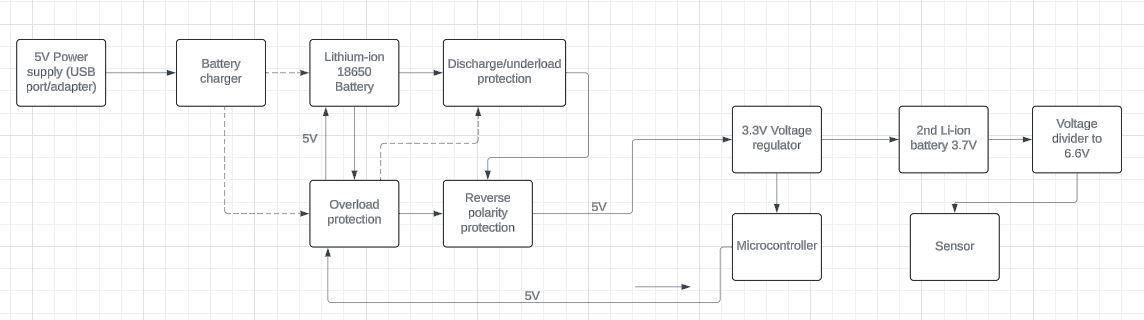
\includegraphics[width=1.2\linewidth]{Figures/flow diagram.jpg}
		\caption{System overview}
		\label{fig:P1}
	\end{figure}
	
	\section{Specifications}
	\subsection{Non-Functional Specifications}
	
	\begin{table}[h!]
		\centering
		\caption{Non-Functional Specifications for Power Subsystem}
		\label{tab:P1}
		\begin{tabularx}{0.9\textwidth}{ 
				| >{\centering\arraybackslash}m 
				| >{\centering\arraybackslash}b 
				| >{\centering\arraybackslash}s |}
			\hline
			\textbf{No.}  & \textbf{Description}                                                                                                     &\textbf{zAcceptance criteria} \\ \hline
			PS1   & Charging compatibility   & The PSU must have a charging system that is easy and compatible to common charging power sources.   \\ \hline
			& PS2 & Safety      & The PSU must be designed in such a way that it provides safety to the users (Sally and and birds), as well as safety to the components used.  \\ \hline
			& PS3  & Physical Size    & The Power supply unit should relatively take less space in the whole design not to scare away the birds. \\ \hline
			& PS4  & Battery monitoring    & The user must be able to easily monitor the battery life of the design. \\ \hline
			
		\end{tabularx}
	\end{table}
	\subsection{Functional Specifications}
		\begin{table}[h!]
		\centering
		\caption{Functional Specifications for Power Subsystem}
		\label{tab:P2}
		\begin{tabularx}{0.9\textwidth}{ 
				| >{\centering\arraybackslash}m 
				| >{\centering\arraybackslash}b 
				| >{\centering\arraybackslash}s |}
			\hline
			\textbf{No.}  & \textbf{Description}                                                                                                     &\textbf{Acceptance criteria} \\ \hline
			PS5   & Output voltage  & The PSU must have a regulated output voltage of 6.6V to power up the microconroller and sensor as required by the Sensing Submodule.   \\ \hline
			& PS6 & Overload Protection  & The PSU must be ensure that each Li-ion battery does not charge to an overload voltage of 4.2V. \\ \hline
			& PS7  & Physical Size    & The Power supply unit should be within the rage 0.15x0.15m . \\ \hline
			& PS8  & Physical Size    & The Power supply unit should be within the rage 0.15x0.15m . \\ \hline
			& PS9  & Physical Size    & The Power supply unit should be within the rage 0.15x0.15m . \\ \hline
			& PS10  & Physical Size    & The Power supply unit should be within the rage 0.15x0.15m . \\ \hline
			& PS11  & Physical Size    & The Power supply unit should be within the rage 0.15x0.15m . \\ \hline
			
		\end{tabularx}
	\end{table}
	
	\section{Design}
	\subsection{Battery charging}
	\vspace{0.5cm}
	Lithium-ion batteries are rechargeable,  The charging circuit should have a stable power supply. This supply can be achieved  by using a wall adapter, USB port, or another power source, such as a power bank. The charging circuit of the 18650 Li-ion batteries uses a BC745 transistor as the driver of the circuit. The circuit diagram is shown below. The circuit takes in a voltage of between 8V - 5V. This circuit is designed to charge one battery at a time, making it more efficient and reliable. The charging circuit has two LED indicators. These LEDs are designed to indicate the level of the battery power when it is plugged to the charger. When the voltage is low, i.e the battery power is low, the RED LED will be much brighter than the GREEN LED. When the voltage now approaches the maximum voltage of 4.2V (actual voltage on a 3.7V Li-ion battery), the green LED dominates the RED and the user can know that the battery is charged. This is a sample and cost effective way to monitor the charging process of the batteries.
	
	
	\begin{figure}[h!]
		\centering
		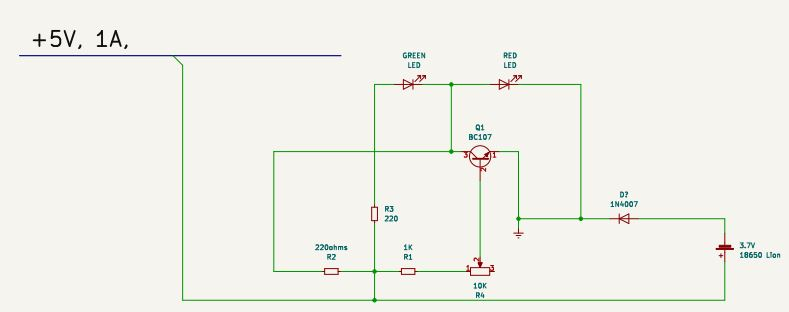
\includegraphics[width=0.9\linewidth]{Figures/Charging.jpg}
		\caption{Charging circuit}
		\label{fig:P2}
	\end{figure}
	\vspace{0.5cm}
	
	
	\subsection{Protection circuitry}
	
	A good design is one which fulfills its requirements and is safe to use. Protection circuitry is necessary in this design to ensure that the device is safe to use as safety plays a huge role in design engineering. Safety also means protection of the components, this will avoid extra costs and time of the user. To avoid burning components, harming the user or even the birds to be scaled, the following protection measures were taken in the design.
	\vspace{0.5cm}
	
	\subsubsection{Overload protection}
	\vspace{0.5cm}
	During the charging process, the 18650 battery must be protected against voltage and current overloading. The overload protection should keep note of key considerations and address to ensure both safety and optimal battery performance. The Li-ion battery has a nominal voltage of 3.7V, it is imperative to note that the specifications of the battery state that the charging voltage should not exceed 4.2V at 0.052A. A common approach involves incorporating a dedicated protection IC that monitors charging parameters such as voltage, current, and temperature. When an overload condition is detected, typically caused by excessive current flow or prolonged charging beyond safe limits, the protection IC triggers a mechanism to shutdown and disconnect the charging circuit from the battery. This prevents overcharging, which can lead to overheating, cell damage, or even fire hazards.
	
	In the circuit below, a 100 ohms resistor was used to limit the current in the base of LM395. Resistors to the values shown below are used to limit the current in the circuit. A power transistor LM395 is used in the overload protection as shown. LM395 is ideal for low power applications such as our small scale sensing design. These transistors act as high gain power transistors, and are capable of power, voltage, current limiting and heat/thermal overloading protection. It is very rare to find a device which is able to provide overload and thermal protection concurrently, which makes the LM395 very reliable to our design. The use of these transistors delivers simplicity and reliability to our design. The thermal limiting circuitry inside the LM395 will terminate the circuit should there be excessive amount of heat, protecting the battery from burning. 
	
	\begin{figure}[h!]
		\centering
		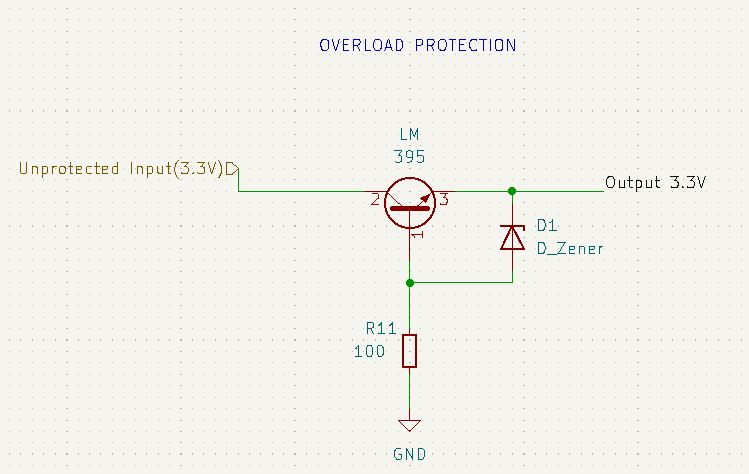
\includegraphics[width=0.9\linewidth]{Figures/Overload protection.jpg}
		\caption{Circuit Schematic of Overload protection}
		\label{fig:P3}
	\end{figure}
	
	\subsubsection{Under voltage protection}
	\vspace{0.5cm}
	As much as the Li-ion batteries need to be protected from overloading conditions, they also need to protection during a discharging process. When the battery is used to power the scale, it gradually discharges as electrical energy is drawn from it. Discharging the battery to 0V damages the battery and reduces its lifespan. To solve this discharge risk, LM358 compactor together with PN2222A, are used in the discharging protection of the battery.The circuitry constantly monitors the battery's voltage level during discharge and charging cycles. When the battery voltage drops below a predefined threshold of 3V, indicating a critically low state of charge, the protection circuit triggers a disconnect mechanism to stop further discharge and protect the battery from damage. This safeguard ensures that the battery remains within safe operating limits, prolonging its lifespan and preventing potentially hazardous conditions. The discharge circuit is shown below. 
	
	\begin{figure}[h!]
		\centering
		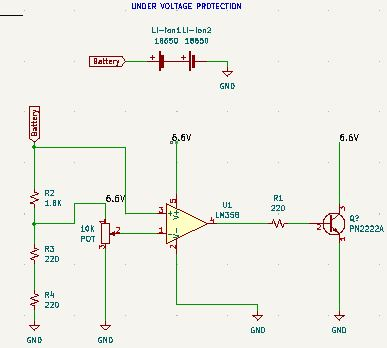
\includegraphics[width=0.9\linewidth]{Figures/ReverseVoltageCircuit.jpg}
		\caption{Circuit Schematic of Under-voltage protection}
		\label{fig:P4}
	\end{figure}
	
	The circuit above shows a voltage divider which divides the battery voltage by a factor of 10. When the batteries' voltage reaches 6V, the circuit cuts off and isolates the battery from the circuit entirely.
	
	\subsubsection{Reverse polarity protection}
	\vspace{0.5cm}
	
	The battery is safeguarded against reverse polarity by employing the a Schottky diode 1N5819. This diode is renowned for its efficacy by having a minimal forward voltage drop of 0.2-0.3V. In the event of reversed battery polarity, the voltage potential at the anode of the diode will be lower than that at the cathode, effectively preventing current flow and thereby shutting the circuit down. No power will be drawn back to the battery, further preserving the battery's lifespan and increasing its reliability. Please see diode's specifications below.
	
	%%instert table of specifications of 1N5819
	
	\subsection{Voltage regulation}
	LM117 was used inthe voltage regulation of the 
	
	
	\begin{figure}[h!]
		\centering
		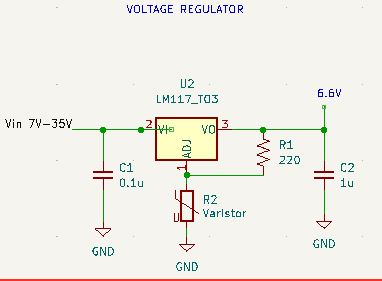
\includegraphics[width=0.9\linewidth]{Figures/regulator.jpg}
		\caption{Charging circuit}
		\label{fig: P1}
	\end{figure}
	
	
	\subsection{Battery power level monitoring}
	To oversee the battery status, a method called voltage divider implementation was employed. This approach entails linking a network of resistors to the battery, establishing a voltage divider setup. The configuration of resistors is engineered to decrease the battery's highest voltage (usually 4.2V for a lithium-ion battery) to a level of voltage that can be precisely gauged by the ESP32's analog pin. By gauging the voltage output of the resistor network, the system can ascertain the remaining charge level of the battery. Subsequently, the ESP32 can enact suitable measures, such as issuing notifications or transitioning into a low-power mode, when the battery's charge level reaches a critical low.
	
	\section{Acceptable Test Procedure}
		\begin{table}[h!]
		\centering
		\caption{Acceptable Test Procedure}
		\label{tab:P3}
		\begin{tabularx}{0.9\textwidth}{ 
				| >{\centering\arraybackslash}m 
				| >{\centering\arraybackslash}b 
				| >{\centering\arraybackslash}s |}
			\hline
			\textbf{No.}  & \textbf{Description}                                                                                                     &\textbf{AAcceptance criteria}
			& Test Result \\ \hline
			ATP1   & Charging compatibility & The PSU must have a charging system that is easy and compatible to common charging power sources. & \textbf{PASSED}  \\ \hline
			& PS2 & Safety      & The PSU must be designed in such a way that it provides safety to the users (Sally and and birds), as well as safety to the components used.  \\ \hline
			& PS3  & Physical Size    & The Power supply unit should relatively take less space in the whole design not to scare away the birds. \\ \hline
			& PS4  & Battery monitoring    & The user must be able to easily monitor the battery life of the design. \\ \hline
			
			PS5   & Output voltage  & The PSU must have a regulated output voltage of 6.6V to power up the microconroller and sensor as required by the Sensing Submodule.   \\ \hline
			& PS6 & Overload Protection  & The PSU must be ensure that each Li-ion battery does not charge to an overload voltage of 4.2V. \\ \hline
			& PS7  & Physical Size    & The Power supply unit should be within the rage 0.15x0.15m . \\ \hline
			& PS8  & Physical Size    & The Power supply unit should be within the rage 0.15x0.15m . \\ \hline
			& PS9  & Physical Size    & The Power supply unit should be within the rage 0.15x0.15m . \\ \hline
			& PS10  & Physical Size    & The Power supply unit should be within the rage 0.15x0.15m . \\ \hline
			& PS11  & Physical Size    & The Power supply unit should be within the rage 0.15x0.15m . \\ \hline
			
		\end{tabularx}
	\end{table}
	\section{Testing and Results}
	
	Battery charging xxxxxxxxxxxxxxxxxxxxxxxxxxxxxxxxxxxxx
	\begin{figure}[h!]
		\centering
		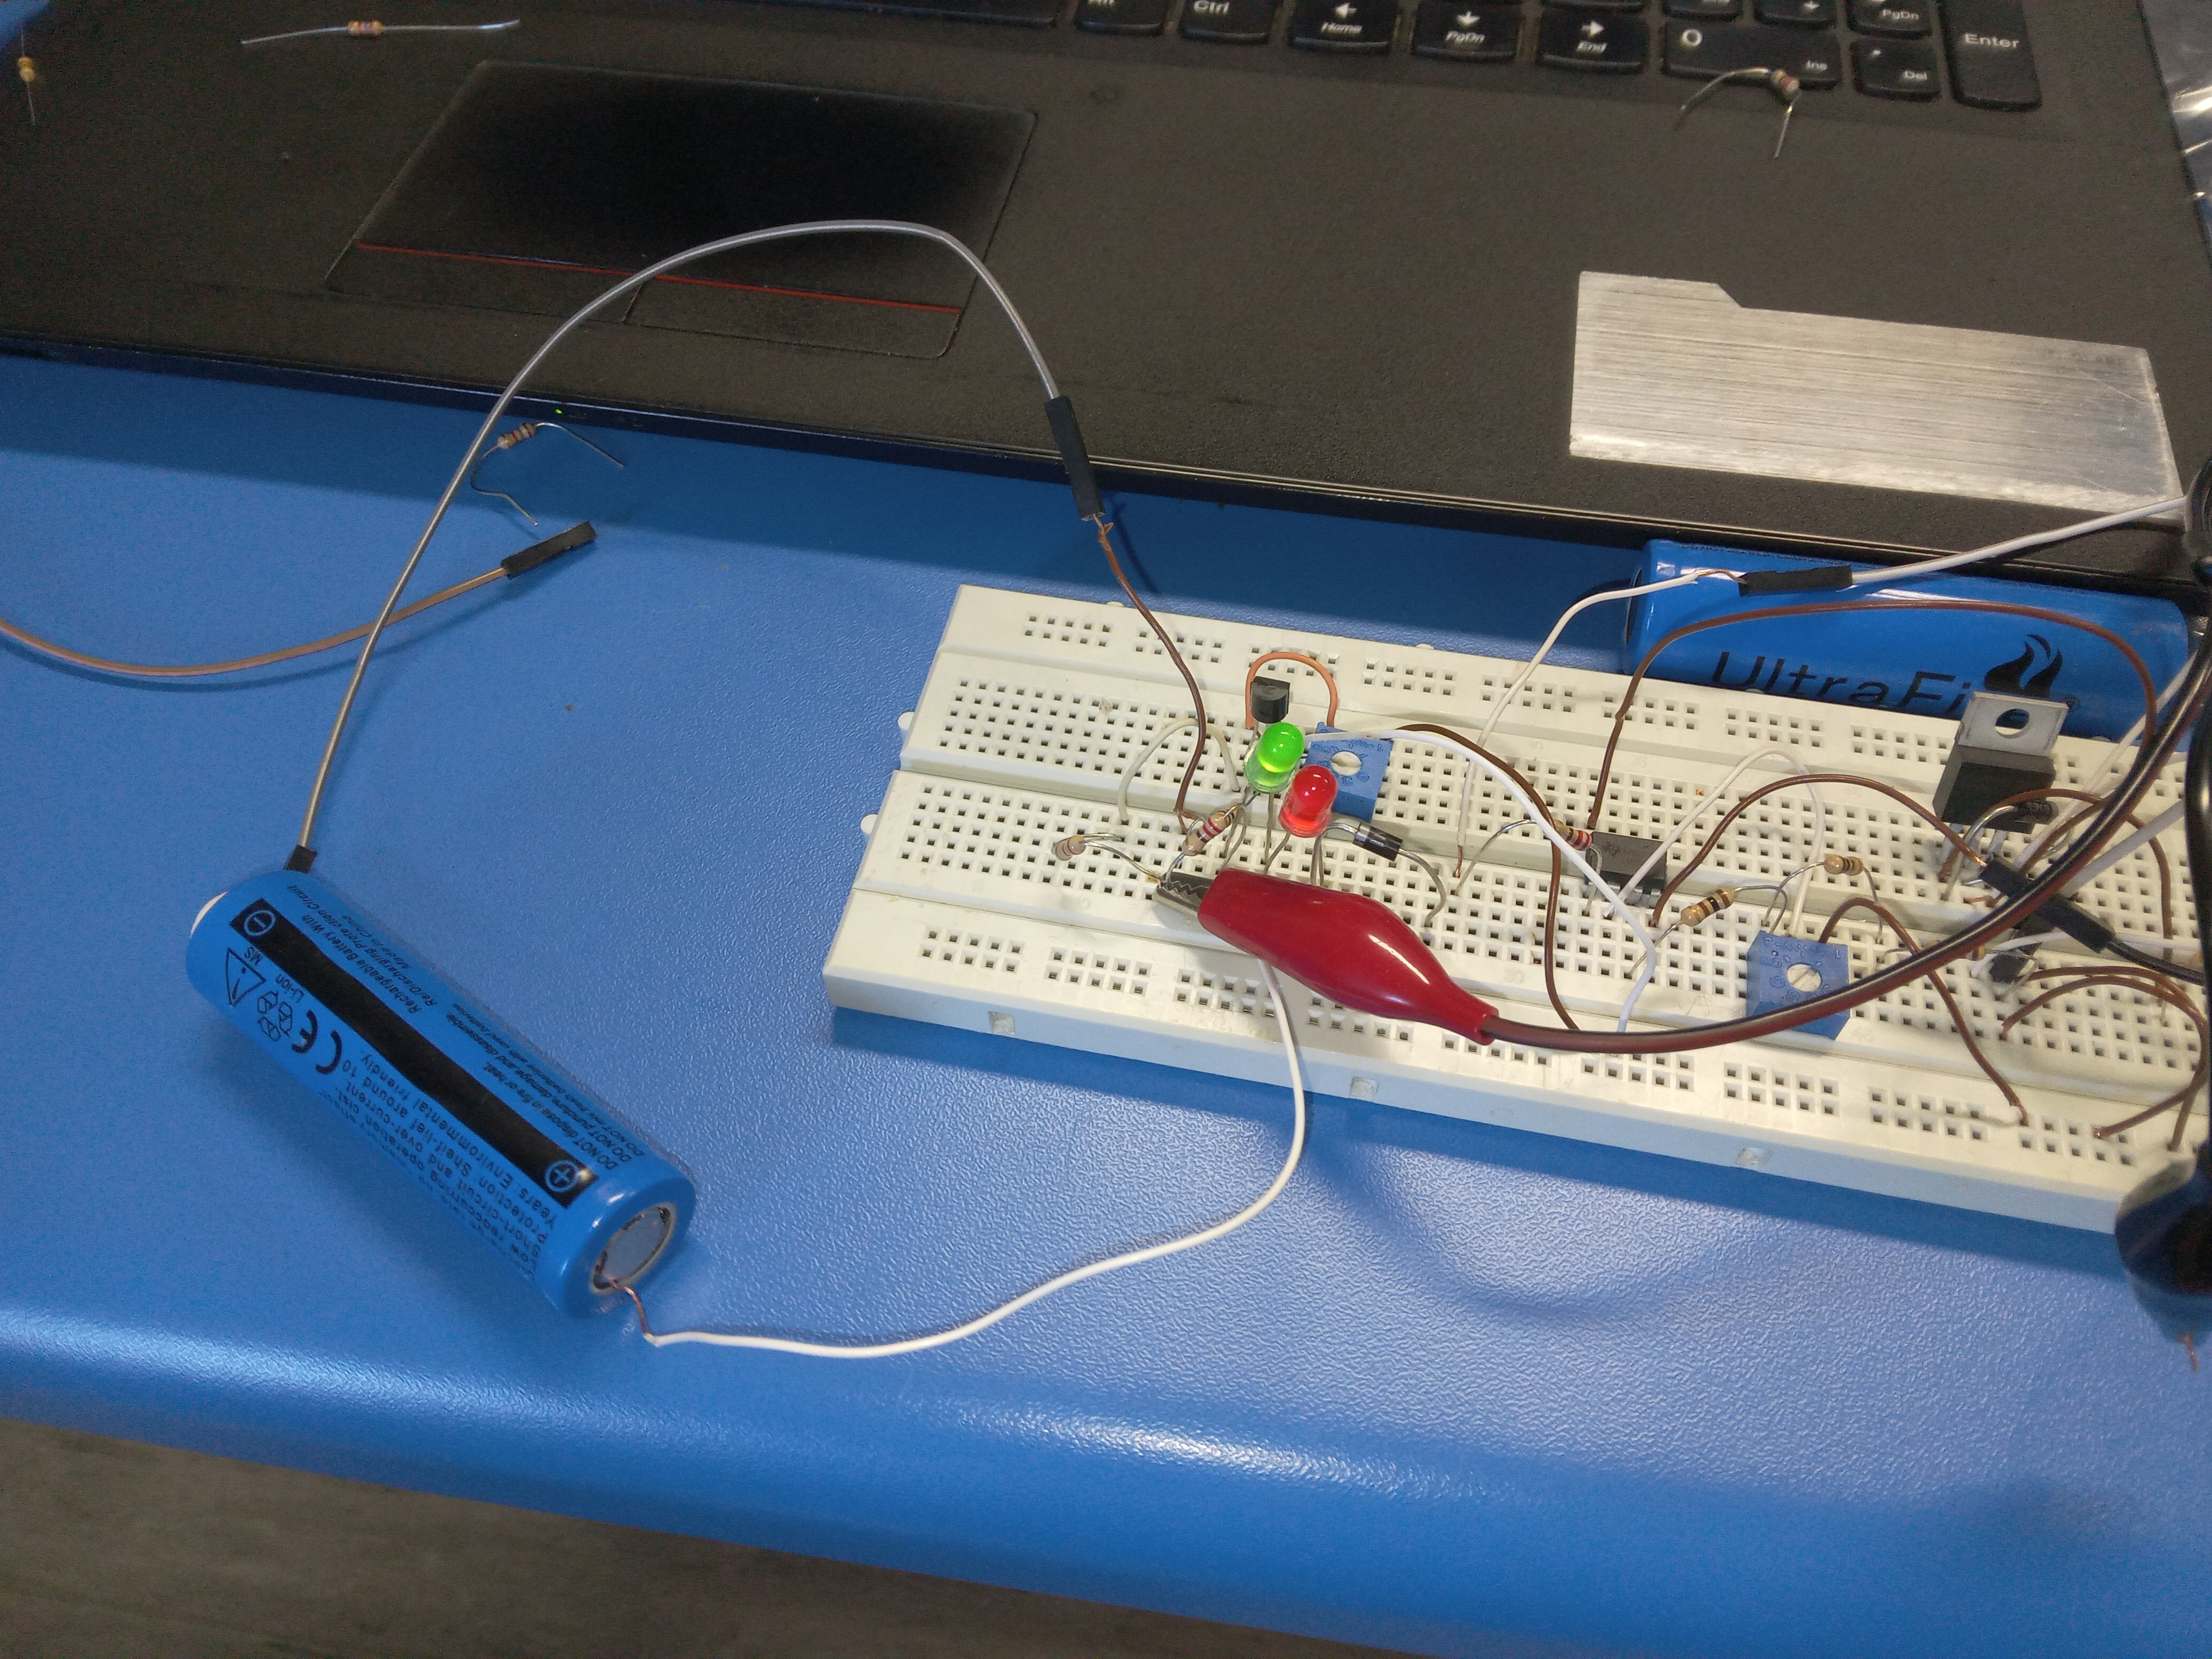
\includegraphics[width=0.8\linewidth]{Figures/Battery chargerG.jpg}
		\caption{Charging circuit}
		\label{fig: P5}
		
	\end{figure}
	
		\begin{figure}[h!]
		\centering
		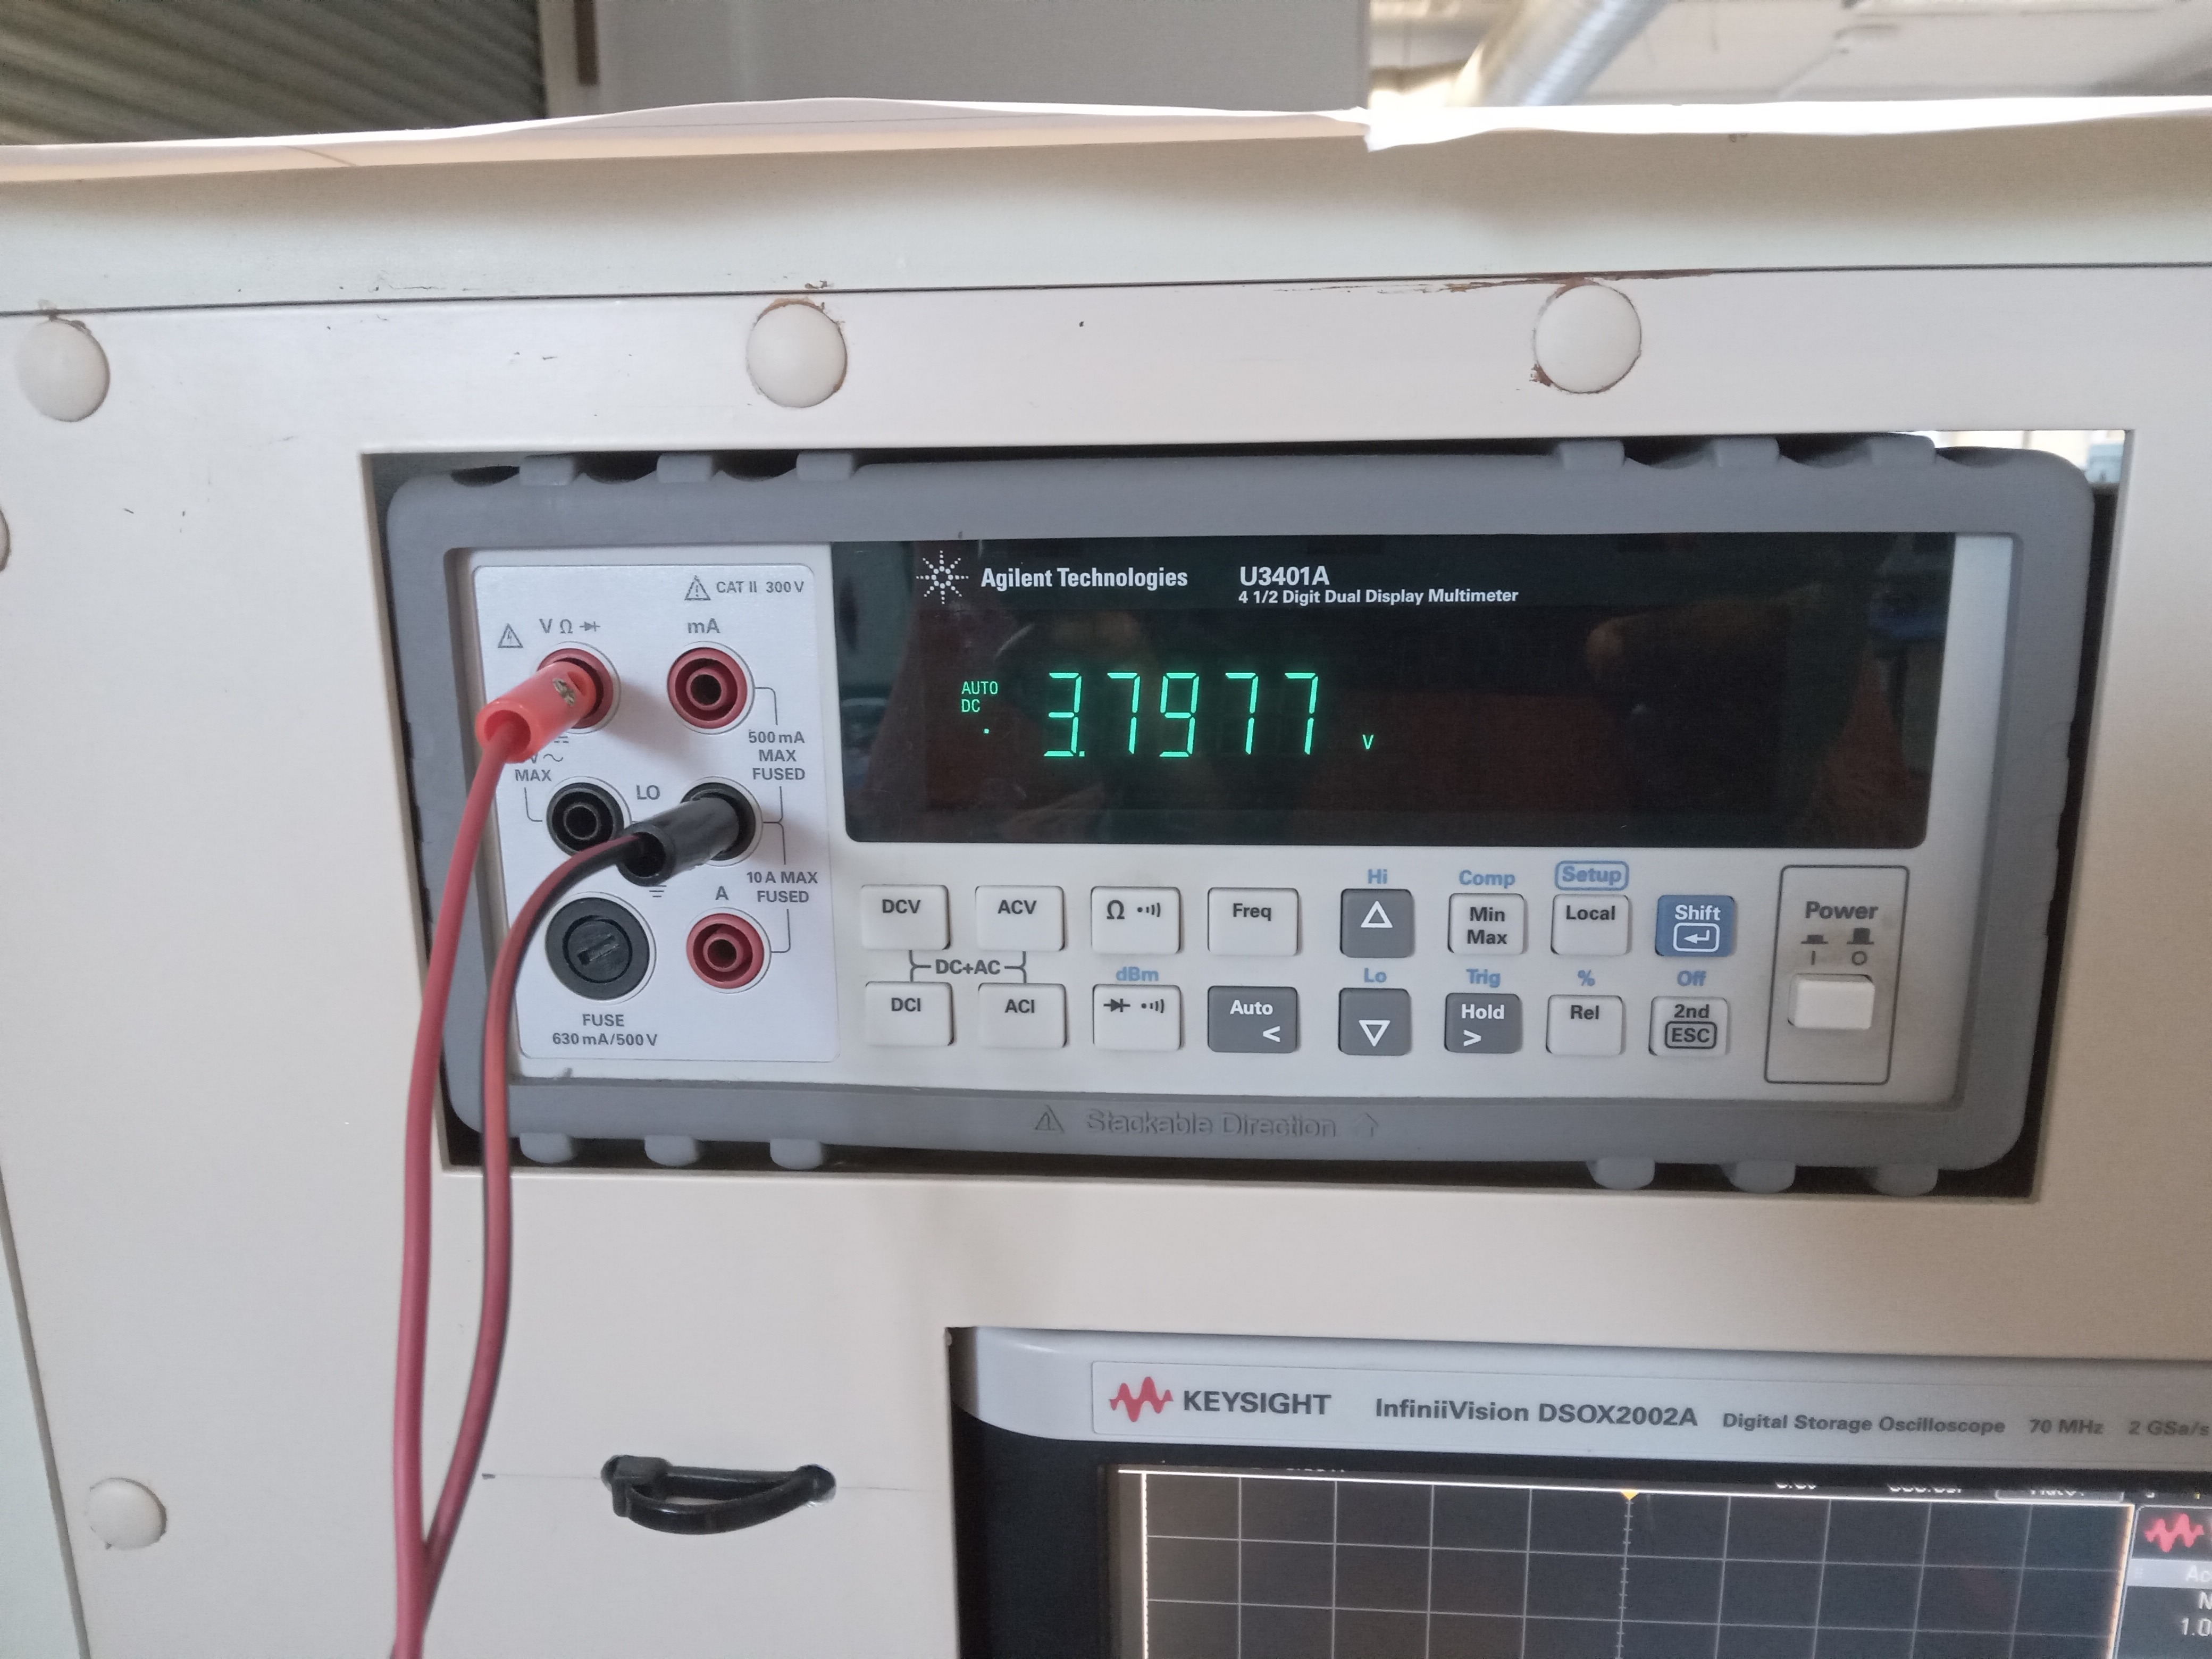
\includegraphics[width=0.8\linewidth]{Figures/Battey voltageC.jpg}
		\caption{Charging circuit}
		\label{fig: P6}
	\end{figure}
	
	
	\begin{figure}[h!]
	\centering
	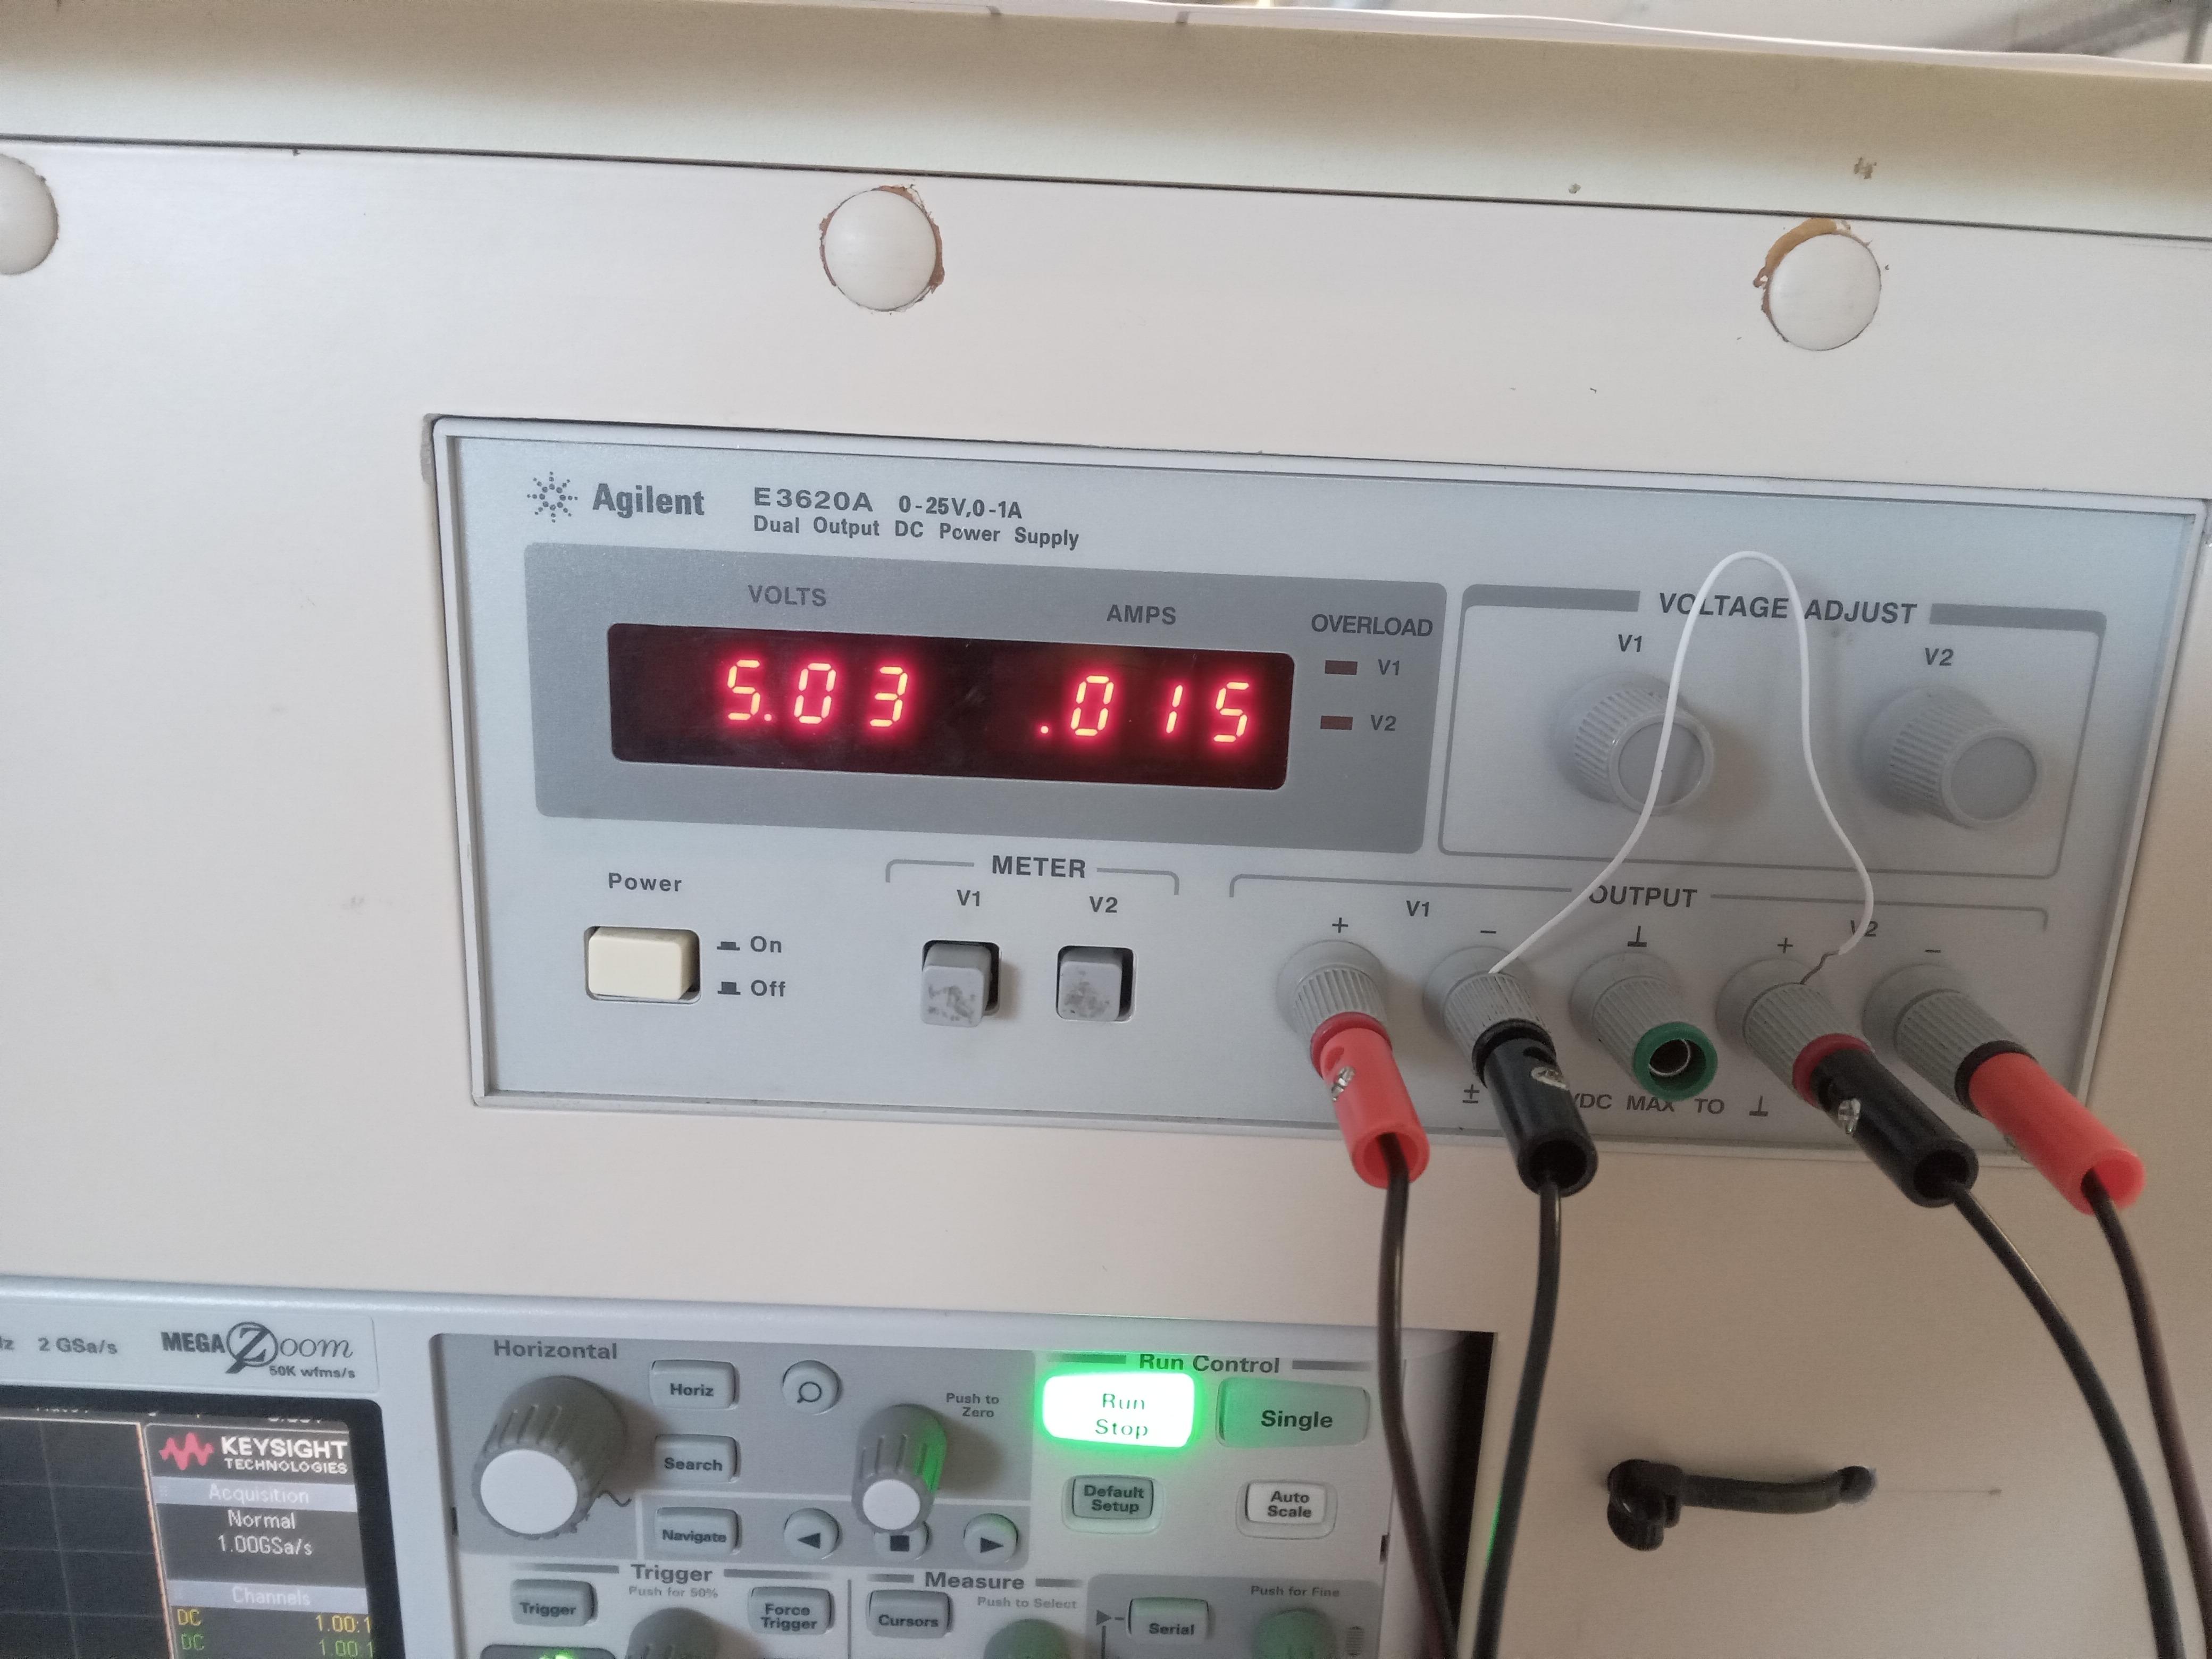
\includegraphics[width=0.8\linewidth]{Figures/Overloading current.jpg}
	\caption{Charging circuit}
	\label{fig: P7}
	\end{figure}
	
	
	Overload and under-load protection xxxxxxxxxxxxxxxxxxxxxxxxxxx
	
	\begin{figure}[h!]
		\centering
		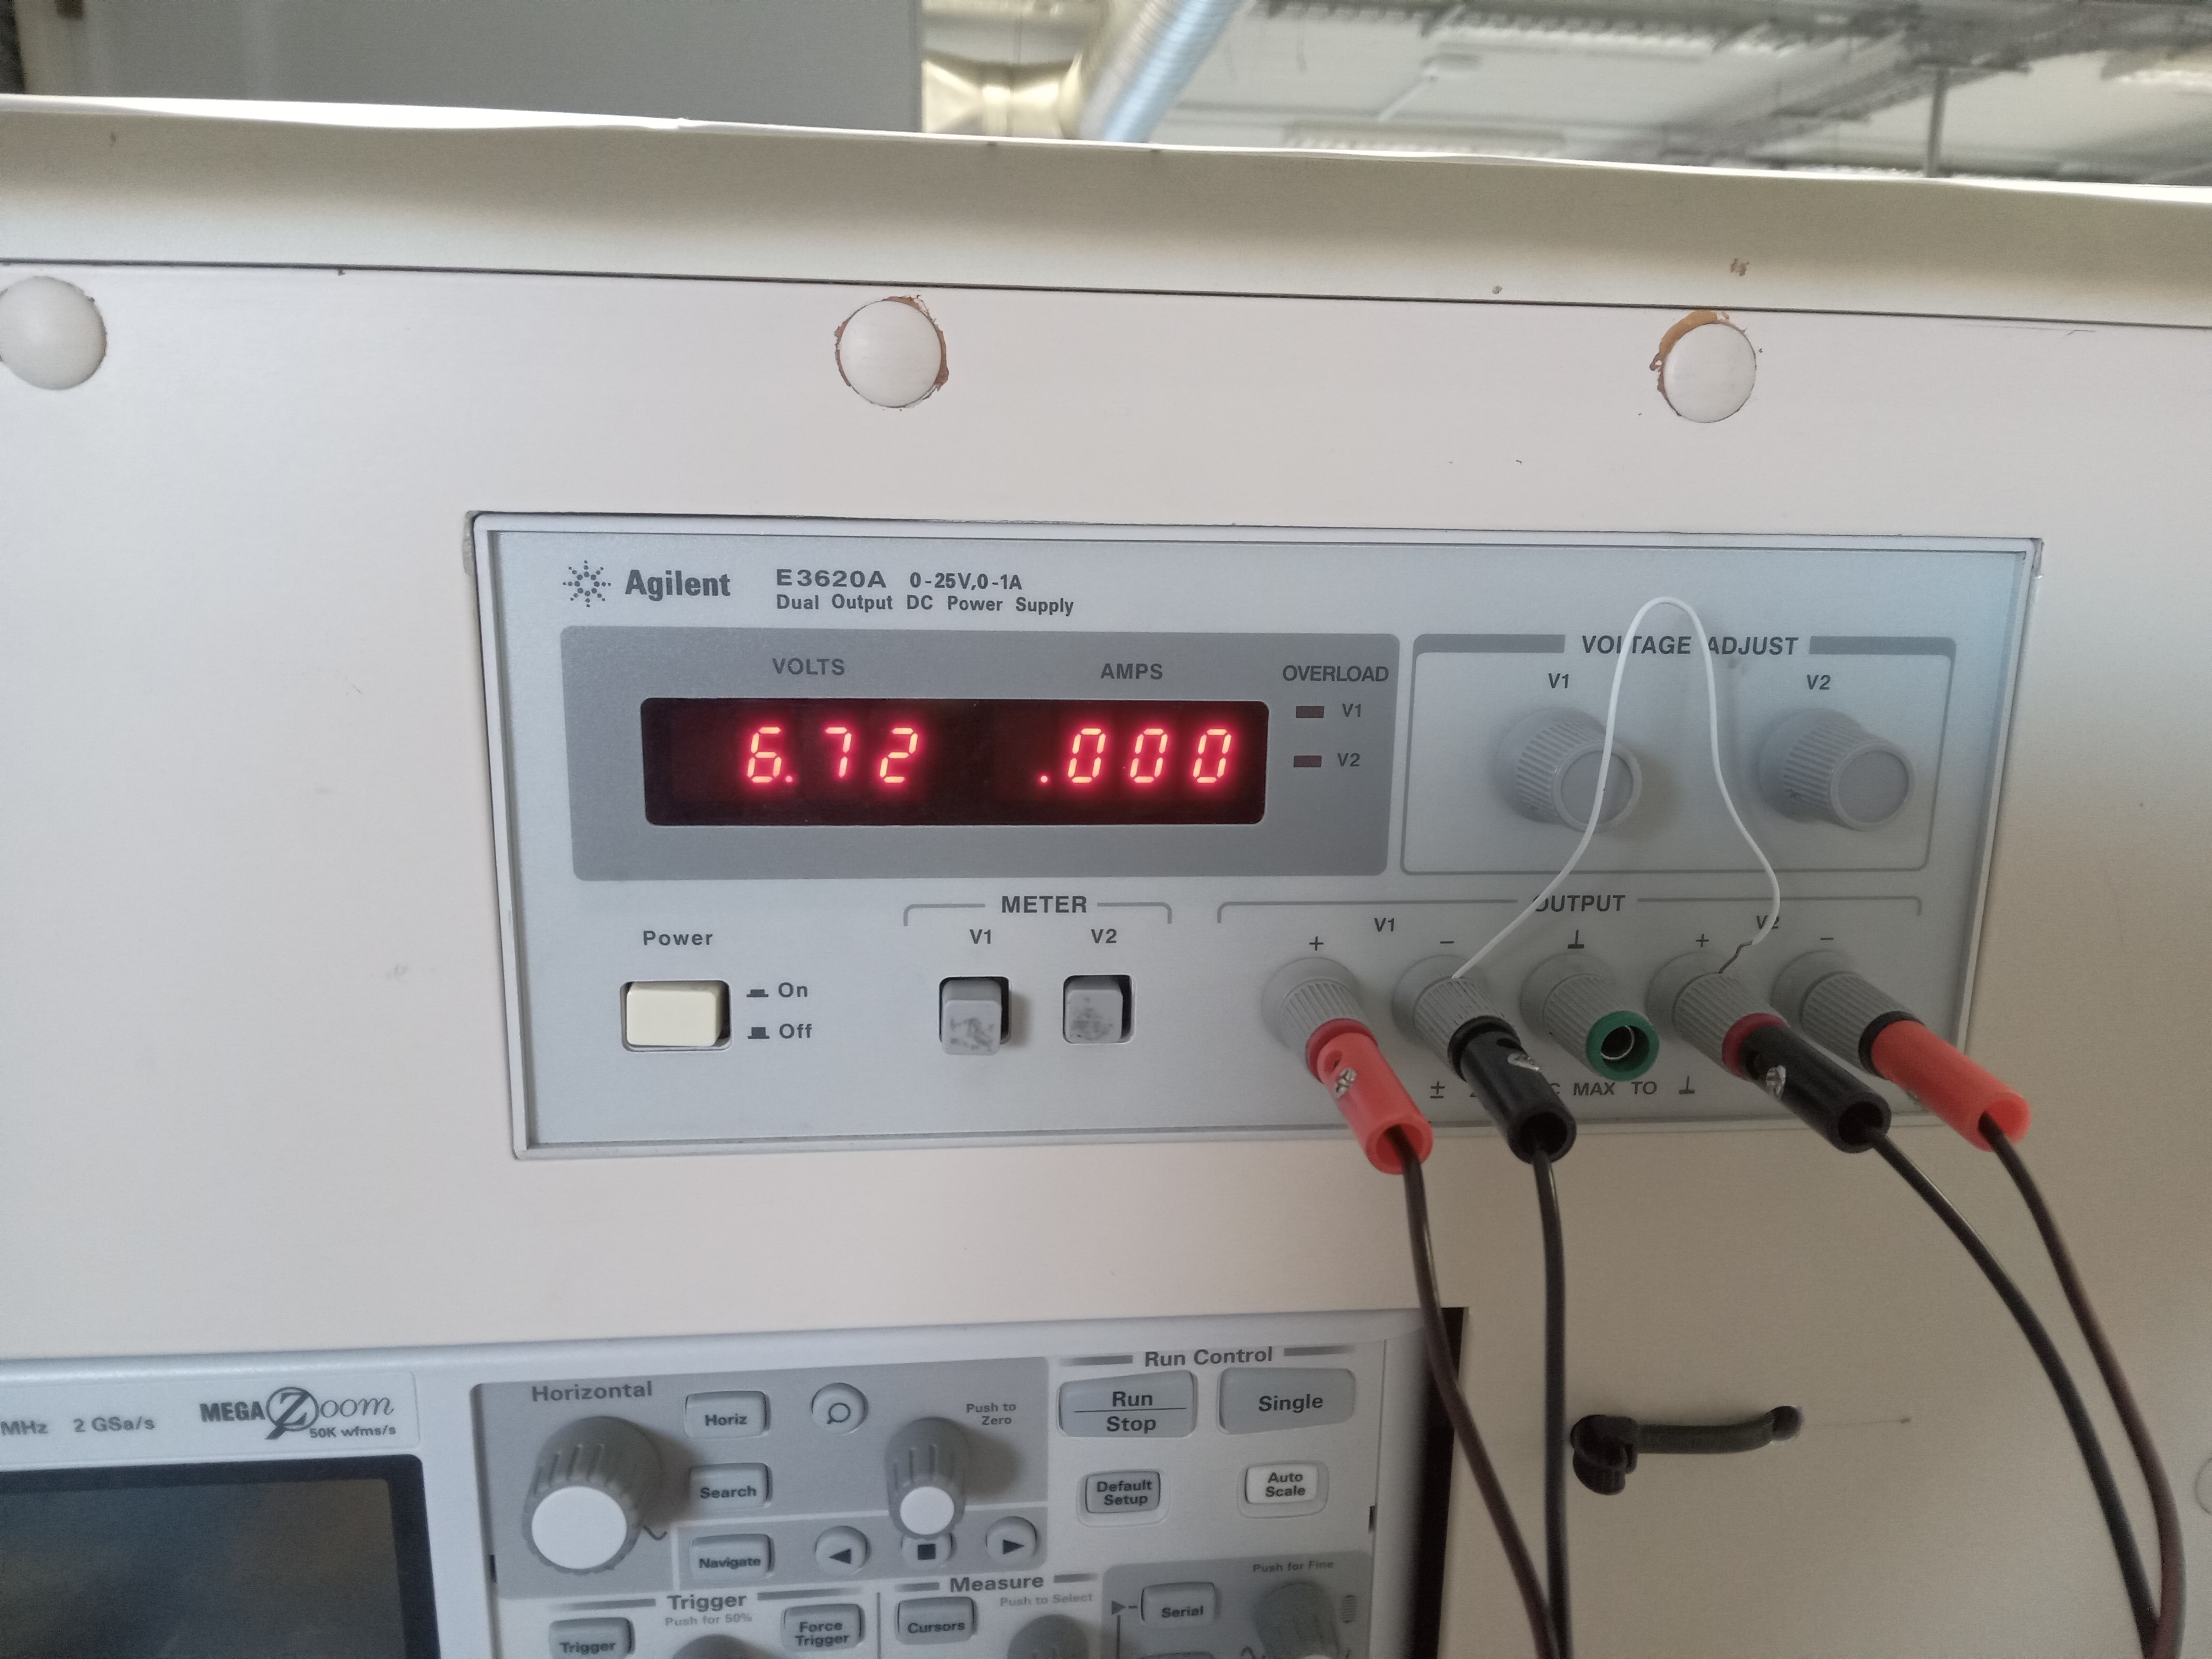
\includegraphics[width=0.8\linewidth]{Figures/OverloadAndUnderloadProtection.jpg}
		\caption{Charging circuit}
		\label{fig: P8}
	\end{figure}
	
	Voltage regulation xxxxxxxxxxxxxxxxxxxxxxxxxxxxxxx
	\section{Conclusion}
	
\end{document}